\usepackage{graphicx}
\graphicspath{ {./images/} }
\begin{document}
\section{Aplicação Móvel}
A aplicação móvel destina-se exlusivamente aos clientes da empresa utilizadora deste serviço. 
A aplicação desenvolvida divide-se em três módulos principais: O módulo de filas, o módulo de senhas
e o módulo de marcações, sendo estes separados por abas. A figura \ref{fig:diam} ilustra as funcionalidades presentes na aplicação móvel.
\begin{figure}[h]
    \centering
    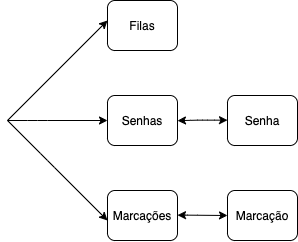
\includegraphics[width=0.25\textwidth]{DiagramaMobileApp}
    \caption{Diagrama de navegação da Aplicação móvel}
    \label{fig:diam}
\end{figure}

A primeira página a ser desenvolvida foi a página do módulo das filas. O principal objetivo desta página é apresentar ao cliente
todas as filas existentes no sistema (nome, assunto e se é uma fila prioritária ou não), em que número vai cada fila e,
ao carregar numa fila, dar a possbilidade ao cliente de tirar uma senha para a mesma. Na figuras \ref{fig:} é possível observar mocks
da página de filas tanto para android como para ios.

\begin{figure}
\centering
\begin{subfigure}{.5\textwidth}
  \centering
  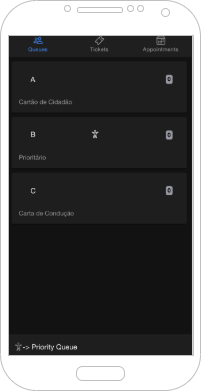
\includegraphics[width=.4\linewidth]{mockQueuesAndroid}
  \caption{Android}
  \label{fig:queuesAndroid}
\end{subfigure}%
\begin{subfigure}{.5\textwidth}
  \centering
  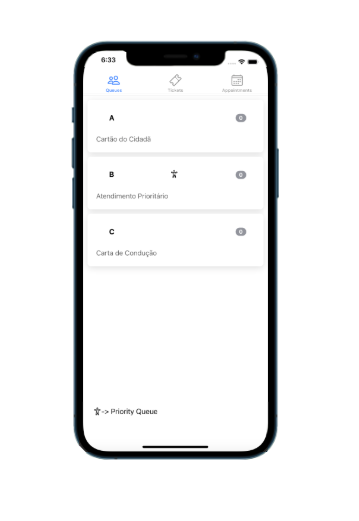
\includegraphics[width=.4\linewidth]{mockQueuesIOS}
  \caption{IOS}
  \label{fig:queuesIos}
\end{subfigure}
\caption{Mock da página das filas}
\label{fig:mockQueues}
\end{figure}
Na página das senhas é apresentada ao cliente uma lista com as suas senhas (com um máximo de uma senha por fila) e, carregando na senha,
o cliente será redirecionado para outra página com os detalhes da mesma, entre as quais, o seu número, o assunto da fila, quantas pessoas
estão à sua frente e em que número vai a fila para a qual tirou senha. Terá também a possbilidade de cancelar a senha em ambas as páginas
deste módulo.

\begin{figure}
\centering
\begin{subfigure}{.5\textwidth}
  \centering
  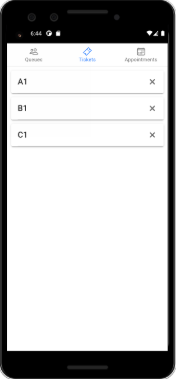
\includegraphics[width=.4\linewidth]{mockTicketsAndroid}
  \caption{Android}
  \label{fig:ticketsAndroid}
\end{subfigure}%
\begin{subfigure}{.5\textwidth}
  \centering
  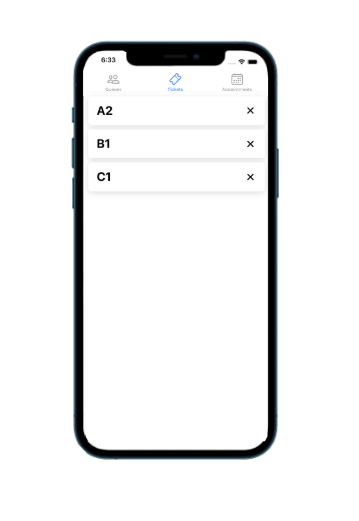
\includegraphics[width=.4\linewidth]{mockTicketsIOS}
  \caption{IOS}
  \label{fig:ticketsIos}
\end{subfigure}
\caption{Mock da página das senhas}
\label{fig:mockTickets}
\end{figure}

\begin{figure}
\centering
\begin{subfigure}{.5\textwidth}
  \centering
  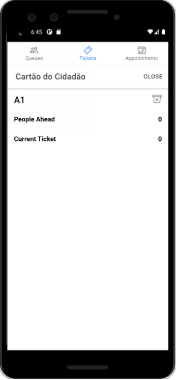
\includegraphics[width=.4\linewidth]{mockTicketDetailsAndroid}
  \caption{Android}
  \label{fig:ticketDetailsAndroid}
\end{subfigure}%
\begin{subfigure}{.5\textwidth}
  \centering
  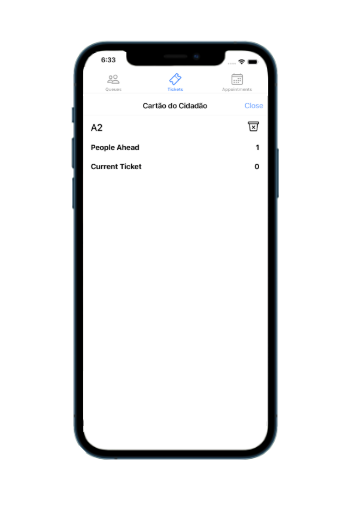
\includegraphics[width=.4\linewidth]{mockTicketDetailsIOS}
  \caption{IOS}
  \label{fig:ticketDetailsIos}
\end{subfigure}
\caption{Mock da página dos detalhes de uma senha}
\label{fig:mockTicketDetails}
\end{figure}

\appendix
\chapter{Documentação das Rotas da API}
\appendix

\chapter{Documentação das Rotas da API}

O URL base desta API é /api. As próximas secções irão descrever cada endpoint da API.

\section{Módulo de Filas}
O Módulo de Filas contem 3 rotas distintas às quais são feitos 5 pedidos diferentes. Nos próximos pontos 
iremos descrever cada um desses pedidos
\subsection{GET /queues}
Este pedido retorna a lista das filas existentes em sistema. Tanto o administrador como os clientes deste sistema tem acesso a este pedido.




\end{document}